\documentclass{article}

\title{Dynamic metacommunity model to evaluate HPV strain interactions}
\author{Joe Mihaljevic}

\usepackage{geometry}
\geometry{legalpaper, portrait, margin=1in}

\usepackage{Sweave}
\begin{document}
\Sconcordance{concordance:ReadMe.tex:ReadMe.Rnw:%
1 8 1 1 0 67 1 1 2 1 0 1 30 31 0 1 2 4 1 1 24 1 2 2 1 1 2 4 0 1 2 1 1 1 %
24 1 2 3 1 1 2 4 0 1 2 1 1 1 24 1 2 3 1 1 2 1 0 1 1 3 0 1 2 1 1 1 34 1 %
2 10 1}

\maketitle

\section*{Introduction}

The goal of this project is to create a dynamic, statistical, metacommunity model. Importantly, the model will allow for and estimate correlations among HPV strains so that hypotheses can be made as to which strains may ecologically interact via priority effects, facilitation, or competition.We will then apply this model to a data set of HPV co-infection dynamics across a large number of patients. The main novelties of this project are: (1) that we have a unique data set with many HPV strains across a large number of patients, and (2) that this is the first stastistical metacommunity model that estimates pair-wise correlations in the probabilities of colonization and persistence.

\section*{Model Specification}

HHere we will outline the dynamic, statistical metacommunity model. This model is based off of Dorazio et al. 2010, Ecology. Importantly, this model does not include the estimation of probability of detection, which corresponds in Dorazio 2010 to the probability of observing rare species. However, detection probability could later be incorporated in our model to reflect the sensitivity and specificity of HPV genotype testing.

Our data set consists of $K$ number of patients, who have been scored for the binomial occupancy of any of $I$ number of HPV strains over $T_{k}$ number of visits, where $T_{k}$ is allowed to vary among patients. Thus the data are of type $y_{ikt}$, which simply consists of a 0 or 1, depending on whether HPV strain $i$ was present in patient $k$ on visit $t$. 

First, we must estimate the initial occupancy probability for each HPV strain, which will then be used in a Markov Process to estimate how strain occupancy changes within and among individuals through time. 
$$y_{ik1} \sim Bern(\psi_{ik1})$$
$\psi_{ik1}$ estimates the probability that strain $i$ occupies patient $k$ at the patient's first visit. The occupancy probabilities for all subsequent visits depend upon the occupancy status of the previous visit, as follows:

$$y_{ik,t+1} \sim Bern(\psi_{ik,t+1})$$
$$\psi_{ik,t+1} = \phi_{ikt}\psi_{ikt} + \gamma_{ikt}(1-\psi_{ikt})$$

In this formulation, the likelihood of a patient retaining HPV strain $i$ from one visit to the next, depends upon the probability of strain $i$ being present at the previous visit, $\psi_{ikt}$, multiplied by the strain-, patient- and time-specific probability of persistence, $\phi_{ikt}$. This persistence probability can also be usefully thought of in terms of an extinction probability, $\xi_{ikt} = 1 - \phi_{ikt}$. Then, the probability that a patient $k$, who is previously uninfected with HPV strain $i$, becomes infected by strain $i$ at time $t+1$ is mediated by the colonization probability, $\gamma_{ikt}$.

\subsubsection*{Covariate effects and induced correlations}

One of our main goals is to determine how strain interactions might affect the ability of a given strain to colonize a new host or to persist in a host. However, we also want to control for the fact that certain strains may respond similarly to certain characteristics of the host environment. For example, if HPV strains A and B both favor young men, we would like to control for this common response when estimating how strain A might affect strain B's colonization probability. In order to account for strain responses to covariates and to simultaneosly estimate covariance among strains, we estimate colonization and persistence probabilities in the following way. For clarity, we will only present the model for persistence probability, although colonization probability is modeled in the exact same way. 

$$ logit(\phi_{ikt}) = \textbf{B}_{i}\textbf{X}_{k} + \textbf{B}^{k}_{i}\textbf{X}_{t[k]} $$

This model is a non-nested multi-level model, because patients have variable numbers of visits and some covariates are measured at the patient level and are static throughout the experiment, while other covariates are dynamic through time. Importantly, the structure of the data makes it easy to incorporate time-varying covariates in this framework, as the full set of covariates are measured at each visit, and time is indexed by visit number. In the above expression, $ \textbf{B}_{i} = (b_{0i}, b_{1i}, \dots, b_{qi})^{'} $ for $q$ number of covariate effects measured at the patient level that do not change across visits. Thus, $ \textbf{X}_{k} = (1, x_{1k}, x_{2k}, \dots, x_{qk}) $ holds the patient-level values of these covariates. We then incorporate a strain-specific, among-patient, random effect via by drawing the intercepts, $b_0$, from a multivariate normal distribution:

$$ b_0 \sim N(\mu_{\phi}, \Sigma_{b_{0}}), $$

where $\mu_{\phi}$ is the overall persistence probability given average covariate values (i.e. global average across strains), and $\Sigma_{b_{0}}$ is a covariance matrix, which accounts for among-patient correlations between strains' persistence probabilities:

$$ \Sigma_{b_{0}} = \left[
                \begin{array}{ccc}
                \sigma_{i}^2 & \dots & \rho_{i,I}\sigma_{i}\sigma_{I} \\
                \vdots & \ddots & \vdots \\
                \rho_{i,I}\sigma_{i}\sigma_{I} & \dots & \sigma_{I}^2
                \end{array}
                \right]
$$
Here $\sigma_{i}^2$ is the variance in persistence probability for strain $i$ across all patient samples. 

The next component of the model contains $ \textbf{B}^{k}_{i} = (b^k_{1i}, b^k_{1i}, \dots, b^k_{ri})^{'} $. These are strain-specific responses to covariates, $(1,...,r-1)$, that were measured at the patient-level. However, these covariates, $ \textbf{X}_{t[k]} = (1, x_{1t[k]}, x_{2t[k]}, \dots, x_{rt[k]}) $, are those covariates which were measured at the patient level and potentially have unique values for each patient visit $t$. Thus, we are able to also account for within-patient correlations between strains' persistence probabilites, similarly:

$$ b^k_1 \sim N(0, \Sigma_{b^k_{1}}), $$
where
$$ \Sigma_{b^k_{1}} = \left[
                \begin{array}{ccc}
                \sigma_{ik}^2 & \dots & \rho_{k_{i,I}}\sigma_{ik}\sigma_{Ik} \\
                \vdots & \ddots & \vdots \\
                \rho_{k_{i,I}}\sigma_{ik}\sigma_{Ik} & \dots & \sigma_{Ik}^2
                \end{array}
                \right]
$$
Here $\sigma_{ik}^2$ is the variance in persistence probability measured within patients for strain $i$ . 

Thus our model estimates both the among-patient and within-patient strain correlations in persistence and colonization probabilities. It is important to distinguish these among- and within-patient effects because the correlations among strains may be scale-dependent, with different processes leading to different patterns between the two scales (i.e. Simpson's paradox). For example, across all patients and visits, strains A and B may have positively correlated colonization probabilities resulting from the fact that both strain A and B tend to only be able to infect immuno-compromised individuals. However, within a patient, the strains' colonization probabilities might be negatively correlated if previous infection with strain A hinders the ability of strain B to superinfect. 

\section*{Simulation as proof of concept}

Here we will embed code and figures that prove that our model works in the sense that we can recover imposed parameters from simulated data. We will also show examples in which correlations among strains' persistence or colonization probabilities change sign depending on whether we look across or within patients. 

Let's start with a simple case with only two HPV strains.
\begin{Schunk}
\begin{Sinput}
> # Basic:
> n.strains <- 2 #number of HPV strains
> n.patients <- 100 #number of patients tested
> n.visits <- rbinom(n.patients, 10, .8) #number of visits per patient,which varies among patients
> n.obs.perpat <- n.strains*n.visits #number of "tests" per patient
> n.obs <- sum(n.obs.perpat) #total number of "tests" (One test per strain per patient per visit)
> # Useful transformation functions:
> Logit <- function(x){
+   log(x) - log(1 - x)
+ }
> AntiLogit <- function(x){
+   exp(x) / (exp(x) + 1)
+ }
\end{Sinput}
\end{Schunk}

We need indices to structure the data set.
\begin{Schunk}
\begin{Sinput}
> # Indices:
> Strain <- rep(c(1,2), times=n.obs/n.strains) #Strain index
> Patient <- NULL
> for(i in 1:n.patients){
+   Patient <- c(Patient, rep(i, times=n.obs.perpat[i]))
+ }
> # Overall visit:
> Visit <- rep(1:sum(n.visits), each=n.strains) 
> # Visit number per patient:
> Visit.Pat <- NULL
> for(i in 1:n.patients){
+   Visit.Pat <- c(Visit.Pat, rep(1:n.visits[i], each=n.strains))
+ }
\end{Sinput}
\end{Schunk}

Now we will simulate the covariates measured per patient, which are either static or dynamic through time. We assume centered and scaled, continuous covariates. We will also assign covariate responses.

\textbf{It is important to note that all rates are on the logit scale.}
\begin{Schunk}
\begin{Sinput}
> # Covariates (centered to mean and scaled to 1 sd):
> q.pat <- 1 #number of covariates measured at the patient-level (but not over time)
> q.time <- 1 #number of covariates measured for each patient at each visit
> X.pat.vals <- NULL
> for(i in 1:n.patients){
+   X.pat.vals <- c(X.pat.vals, rep(rnorm(1,0,1), times=n.obs.perpat[i]))
+ }
> X.time.vals <- NULL
> for(i in 1:n.patients){
+   X.time.vals <- c(X.time.vals, rep(rnorm(n.visits[i],0,1), each=n.strains))
+ }
> # Covariate responses:
> b.pat.mean <- .15
> b.time.mean <- .15
> beta.pat <- rnorm(n.strains, b.pat.mean, .75)
> beta.time <- rnorm(n.strains, b.time.mean, .75)
\end{Sinput}
\end{Schunk}

Here we code the across-host strain correlations in persistence and colonization probabilities
\begin{Schunk}
\begin{Sinput}
> #Because we only have 2 strains I will code the
> #covariance matrices manually.
> 
> #Across-patient std.dev. in persistence for each strain:
> sig.across.phi.1 <- .4
> sig.across.phi.2 <- .4
> #Correlation:
> rho.across.phi <- .7
> #Covariance matrix:
> Sig.across.phi <- matrix(
+   c(sig.across.phi.1^2, rho.across.phi*sig.across.phi.1*sig.across.phi.2,
+     rho.across.phi*sig.across.phi.1*sig.across.phi.2, sig.across.phi.2^2),
+   ncol=2
+   )
> #Across-patient std.dev. in colonization for each strain:
> sig.across.gam.1 <- .4
> sig.across.gam.2 <- .4
> #Correlation:
> rho.across.gam <- .5
> #Covariance matrix:
> Sig.across.gam <- matrix(
+   c(sig.across.gam.1^2, rho.across.gam*sig.across.gam.1*sig.across.gam.2,
+     rho.across.gam*sig.across.gam.1*sig.across.gam.2, sig.across.gam.2^2),
+   ncol=2
+   )
> ##############################
> # Within-patient covariances:
> 
> #Within-patient std.dev. in persistence for each strain:
> sig.within.phi.1 <- .2
> sig.within.phi.2 <- .2
> #Correlation:
> rho.within.phi <- -.8
> #Covariance matrix:
> Sig.within.phi <- matrix(
+   c(sig.within.phi.1^2, rho.within.phi*sig.within.phi.1*sig.within.phi.2,
+     rho.within.phi*sig.within.phi.1*sig.within.phi.2, sig.within.phi.2^2),
+   ncol=2
+   )
> #within-patient std.dev. in colonization for each strain:
> sig.within.gam.1 <- .2
> sig.within.gam.2 <- .2
> #Correlation:
> rho.within.gam <- -.6
> #Covariance matrix:
> Sig.within.gam <- matrix(
+   c(sig.within.gam.1^2, rho.within.gam*sig.within.gam.1*sig.within.gam.2,
+     rho.within.gam*sig.within.gam.1*sig.within.gam.2, sig.within.gam.2^2),
+   ncol=2
+   )
> 
> 
\end{Sinput}
\end{Schunk}

Now we'll draw the random effects from the covariance matrices.
\begin{Schunk}
\begin{Sinput}
> library(mnormt) #needed for multivariate normal distrib.
> b.0.phi <- rmnorm(n.patients, mean=rep(0,n.strains), varcov=Sig.across.phi) 
> b.0.gam <- rmnorm(n.patients, mean=rep(0,n.strains), varcov=Sig.across.gam)
> b.1t.phi <- rmnorm(sum(n.visits), mean=rep(0,n.strains), varcov=Sig.across.phi)
> b.1t.gam <- rmnorm(sum(n.visits), mean=rep(0,n.strains), varcov=Sig.across.phi)
> 
\end{Sinput}
\end{Schunk}

We will create vectors of all $\phi$ and $\gamma$ values, one valcue for each observation. 
\begin{Schunk}
\begin{Sinput}
> # Storage:
> phi <- NULL
> gam <- NULL
> # We need to assign the global mean values for phi and gamma
> mean.phi <- Logit(.5)
> mean.gam <- Logit(.5)
> # Formula from our model:
> # (phi/gamma) <- global_mean + intercept_among + covariate_among + 
> #                     intercept_within + covariate_within
> for(i in 1:n.obs){
+   phi[i] <- mean.phi + b.0.phi[Patient[i],Strain[i]] + beta.pat[Strain[i]] * X.pat.vals[i] + 
+                 b.1t.phi[Visit[i],Strain[i]] + beta.time[Strain[i]] * X.time.vals[i]
+   gam[i] <- mean.gam + b.0.gam[Patient[i],Strain[i]] + beta.pat[Strain[i]] * X.pat.vals[i] + 
+                 b.1t.gam[Visit[i],Strain[i]] + beta.time[Strain[i]] * X.time.vals[i]
+ }
> 
\end{Sinput}
\end{Schunk}

Now we can calculate the probabilities of occurrence, $\psi$.
\begin{Schunk}
\begin{Sinput}
> # First we need the initial occurrence probability for each strain for each patient.
> # We assume this probability is not influenced by covariates, but this assumption
> # could be relaxed in the future. Instead we assume the initial probabilities are
> # generated randomly from a global occurrence probability.
> 
> psi.mean <- Logit(.6)
> # Calculate AntiLogit for phi and gam
> lphi <- AntiLogit(phi)
> lgam <- AntiLogit(gam)
> psi <- NULL
> for(i in 1:n.obs){
+   
+   if(Visit.Pat[i]==1){ # If it's the patient's first visit
+     psi[i] <- AntiLogit(rnorm(1,psi.mean,.2))
+   }else{
+     psi[i] <- lgam[i-1] * psi[i-1] + lphi[i-1] * (1 - psi[i-1]) 
+   }
+   
+ }
> 
\end{Sinput}
\end{Schunk}

Finally, to complete the simulation, we will draw observed occurrences from the derived probabilities of occurrence, $\psi$. The benefit of conducting the simulation in the way we did above, is that now we can vectorize the simulated observations. This will be very helpful for optimizing the \emph{stan} model later on.
\begin{Schunk}
\begin{Sinput}
> Y <- NULL
> Y <- rbinom(n.obs, 1, psi)
> # Create a data.frame
> Occ <- data.frame(Y, Strain, Patient, Visit.Pat, X.time.vals, X.pat.vals)
\end{Sinput}
\end{Schunk}

Sometimes, interesting patterns can emerge at the across-patient scale that deviate from the simulated parameters. For instance, if ignored, within-host correlations can strongly bias the estimated among-host covariate effects.
\begin{center}
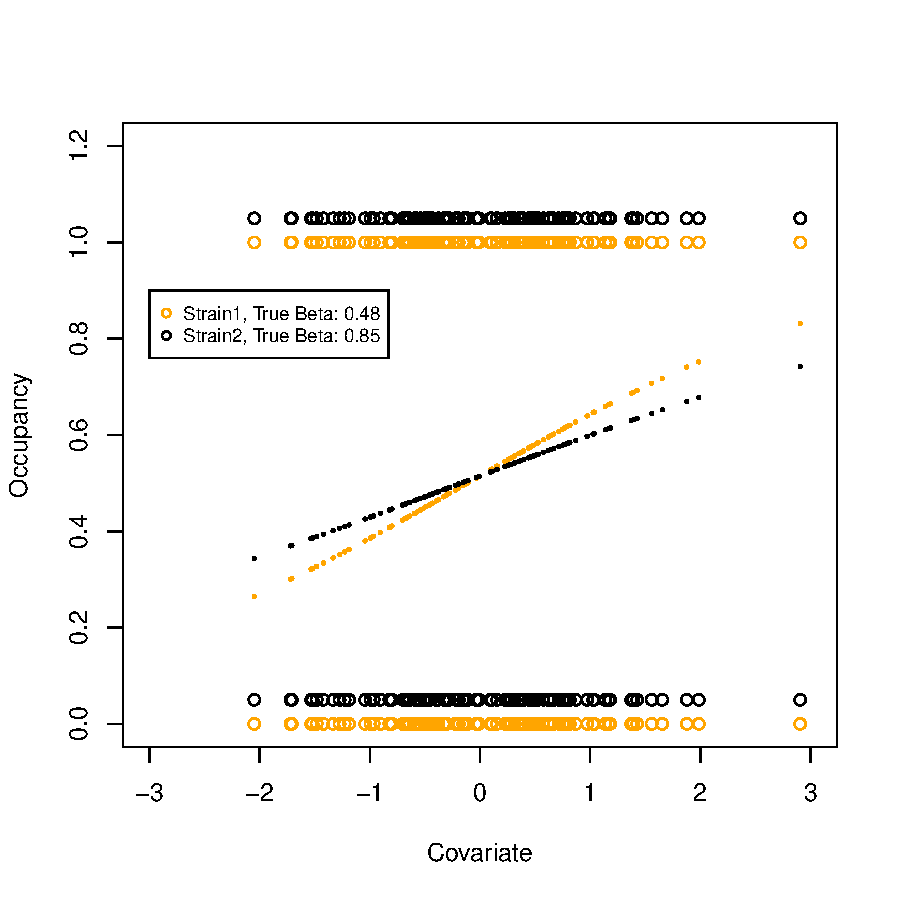
\includegraphics{ReadMe-009}
\end{center}

Now we need to write the \emph{stan} model and make sure that the model can adequately estimate the imposed parameters. 

\end{document}






